\section{Photometry}\label{s: fotometria}

In order to simplify the inputs fed into the filter, it becomes neccessary to obtain simulation-based measurements that faithfully capture the underlying physics of the problem. To achieve this objective, a dedicated photometry module has been implemented, facilitating the computation of key variables such as the apparent magnitude $m$ and the pointing vector towards the Resident Space Object (RSO), denoted as  $\mathbf{d}$ . These variables essentially serve as quantifications of the solar illumination reflected by the facets of the RSO, encapsulating both the magnitude and directional characteristics of the reflected light. 

\subsection{Reflexion model}
With the aim of getting information about the sunlight reflection, it will be necessary to ascertain its geometry. In this project, the targets are characterized as a discrete set of planar facets, each defined by a basis of orthogonal unit vectors ($\mathbf{u}_{n}^{B}, \mathbf{u}_{u}^{B}, \mathbf{u}_{\nu}^{B}$), elucidated in Figure \ref{fig:geom-reflex}. As depicted in this illustration, the basis is determined by the normal vector to the facet ($\mathbf{u}_{n}^{B}$) and two additional vectors lying in the plane of the facet and orthogonal to each other ($\mathbf{u}_{u}^{B}, \mathbf{u}_{\nu}^{B}$), expressed in body-fixed axes denoted by the superscript $B$. This discrete representation provides a comprehensive characterization of the target's geometry, forming the basis for subsequent computations related to sunlight reflection.

\begin{figure}[H]
    \centering
    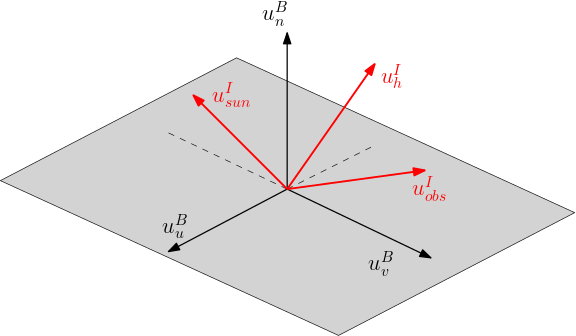
\includegraphics[width=0.6\textwidth]{Figures/Geom_reflexion.png}
    \caption{Geometría de la reflexión}
    \label{fig:geom-reflex}
\end{figure}

In addition, in order to obtain the value of the apparent magnitude, it is needed to model the light curve. This entails having the vectors that define the target's facets in inertial coordinates, denoted by the superscript $I$. To achieve this, the attitude matrix defined by the quaternion associated with the satellite at each moment is employed:

\begin{equation}
\mathbf{u}_k^b = A(\mathbf{q_I^B})\mathbf{u}_k^I, \quad k = u, v, n,
\end{equation}

Simultaneously, it is fundamental to determine the vector representing the sun with respect to the target, $\mathbf{u}_{\text{sun}}^I$, and the vector depicting the target's orientation concerning the observer, $\mathbf{u}_{\text{obs}}^I$.

With the directions of the reflected light with respect to the inertial frame defined, it is now possible to ascertain the variables that the observer will be able to see.

\subsection{Observation model}
Consider that the observing satellite is in a position $\boldsymbol{r_{obs}}$, capable of measuring the azimuth and elevation of the target, $\boldsymbol{r_{RSO}}$. The pointing vector from the observer to the RSO is defined as:
\begin{equation}
    \boldsymbol{d}=\boldsymbol{r_{RSO}}-\boldsymbol{r_{obs}}
\end{equation}

Furthermore, assume that the observer's sensors can measure the magnitude of the reflected light, modeled using the Phong light diffusion model \cite{Phong}, based on the Bidirectional Reflectance Distribution Function (BDRF). In this reference, the authors decompose the BDRF into a specular part (with a preferred direction), $\rho_{spec}$, and a diffuse part, $\rho_{diff}$:
\begin{equation}
    \rho_{tot}(i)=\rho_{spec}(i)+\rho_{diff}(i)\quad i=1...n_c,
\end{equation}
where $n_c$ is the number of facets of the RSO. Assuming flat faces, the specular part of the distribution results in:
\begin{equation}
    \rho_{\mathrm{spec}}(i)=C_{\mathrm{spec}}\frac{(\mathbf{u_{obs}^{I}}\cdot\mathbf{u_{spec}^{I}})}{(\mathbf{u_{sun}^{I}}\cdot\mathbf{u_{n}^{I}})},
\end{equation}
where the vector $\mathbf{u_{spec}^{I}}$ is the preferred direction of specular reflection, defined as $\mathbf{u_{spec}^{I}}=2(\mathbf{u_{n}^{I}}\cdot\mathbf{u_{sun}^{I}})\mathbf{u_{n}^{I}-u_{sun}^{I}}$. On the other hand, the diffuse term results in:
\begin{equation}
    \rho_{diff}(i)=\frac{C_{diff}}{\pi}.
\end{equation}
where $C_{spec}$ and $C_{diff}$ are reflection coefficients dependent on the RSO's surface material.

As the apparent magnitude is the measure reaching the observer's sensors of the light reflected by the RSO, the first step is to calculate the fraction of (visible) light reaching the RSO:
\begin{equation}
    F_{\mathrm{sun}}(i)=\Phi_{\mathrm{sun,vis}}\rho_{\mathrm{total}}(i)(\mathbf{u}_{n}^{I}(i)\cdot\mathbf{u}_{\mathrm{sun}}^{I}),
\end{equation}
where $\Phi_{\mathrm{sun,vis}}$ is the power per unit area received by an object illuminated by sunlight. Only a fraction of the light reflected by the RSO is visible to the observer:
\begin{equation}
    F_{\mathrm{obs}}(i)=\frac{F_{\mathrm{sun}}(i)\mathcal{A}(i)(\mathbf{u}_{n}^{I}(i)\cdot\mathbf{u}_{\mathrm{obs}}^{I})}{\|\mathbf{d}^{I}\|^2}.
\end{equation}

Finally, the apparent magnitude is given by a sum of the fraction of light the observer receives from each of the facets  the RSO :
\begin{equation}
    m_{\mathrm{app}}=-26.7-2.5\log_{10}\left|\sum_{i=1}^{N_{F}}\frac{F_{\mathrm{obs}}(i)}{\Phi_{\mathrm{sun,vis}}}\right|.
    \label{eqn:mapp}
\end{equation}

Note that, for the RSO to reflect light, it must be illuminated by sunlight, meaning that the periods of eclipse need to be restricted. Furthermore, if either the angle between the surface normal and the observer or the angle between the surface normal and the Sun direction is greater than $\pi/2$ the observer will not receive any light from this surface. 

These calculations have been implemented in the simulator through the \textit{magnitude\_apparent.m} function, presented below:

% \begin{lstlisting}[language=Matlab, caption= Excerpt of function \textit{magnitude\_apparent.m}.]
   
%     function mapp = magnitude_apparent1(ro_vir, rt, rsun, qt, SO)
%     phi_sun_vis = 455;
%     alpha = 1;
%     Rt=6378e3;

%     % Number of observers
%     n_observers = size(ro_vir, 1);

%     for j = 1:n_observers
       
%         % Vector from observer to target
%         d = rt' - ro_vir(j, :);
%         % Normalize vectors
%         u_obs_I = normr(-d);
%         u_sun_I = normr(rsun - rt');

%         % Check if the target is in eclipse
%         angle_target_sun = real(acos(dot(rt, rsun)/(norm(rsun) * norm (rt))));
%         eclipse_angle = asin(Rt/norm(rt));
%         if angle_target_sun > (pi-eclipse_angle) || (angle_target_sun < (eclipse_angle + pi) && angle_target_sun > (pi-eclipse_angle))
%             % Target is in eclipse, set solar flux to zero
%             fobs = 0;
            
%         else
%             % Initialize apparent magnitude
%             fobs = 0;

%             % Loop over surface elements
%             for k = 1:6
%                 % Rotate surface normal to inertial frame
%                 u_n_I = (quat2rotm(qt') * SO.Normals(k, :)')';

%                 % Compute angles between surface normal, observer's direction, and Sun direction
%                 angle_obs = acos(dot(u_n_I, u_obs_I));
%                 angle_sun = acos(dot(u_n_I, u_sun_I));

%                 % Check if either angle is greater than pi/2
% %                 if (angle_obs > pi/2 && angle_obs < 3*pi/2) || (angle_sun > pi/2 && angle_sun < 3*pi/2)
% %                     % No light reflected toward the observer
% %                     fsun = 0;
% %                     break
% %                 else
%                     % Compute reflected and diffuse components
%                     u_esp_I = 2 * dot(u_n_I, u_sun_I) * u_n_I - u_sun_I;
%                     rho_esp = SO.Cesp(k) * dot(u_obs_I, u_esp_I)^alpha / dot(u_sun_I, u_n_I);
%                     rho_dif = SO.Cdif(k) / pi;

%                     % Compute solar flux
%                     fsun = phi_sun_vis * (rho_dif + rho_esp) * dot(u_n_I, u_sun_I);
% %                 end

%                 % Accumulate flux from each surface element
%                 fobs = fsun * SO.Areas(k) * dot(u_n_I, u_obs_I) / norm(d)^2 + fobs;
%             end
%         end

%         % Calculate apparent magnitude for the observer
%         mapp(j) = -26.7 - 2.5 * log10(fobs / phi_sun_vis);
%     end
% end
% \end{lstlisting}

From this function, a significant portion of the results presented in Section \ref{s: resultados} has been derived. The \textit{magnitude\_apparent.m} function, described earlier, has played an important role in computing various outcomes that contribute to the findings detailed in the subsequent section. 

